\chapter{Desarrollo de prototipos}
\label{cap:Desarrollo de prototipos}
El presente capítulo tiene como objetivo contar, en orden temporal, como ha sido la construcción del chatbot de ayuda a la terapia de reminiscencia. Así, habla sobre los detalles, características y las tecnologías involucradas en cada uno de los prototipos que han llevado el proyecto hasta el prototipo final. 
%PRIMERA VERSIÓN EN BARD
%PRIMERA VERSIÓN EN GEMMA
%PRIMERA VERSIÓN GEMINI - GOOGLE COLLABORATE
%REFACTORIZACIÓN PARA HACER VERSIÓN LOCAL
%TELEGRAM
%GENERAR LAS ETAPAS 
%IMAGENES
%WHISPER
%GRÁFOS
%GENERACIÓN DE HISTORIAS DE VIDA

\section{Prototipo con preguntas predefinidas}
%Parsea la información utilizando BARD
\section{Prototipo con preguntas predefinidas usando Gemma}
\section{Prototipo con preguntas predefinidas usando}
\section{Gemini}
\section{Gemini preguntas}
\section{Gemini almacenamiento de información}
Como se puede ver en la figura \ref{fig:interfazPYQT5} estas bibliotecas permiten crear interfaces bastantes usables y simples. Sin embargo, aunque la interfaz es de buena calidad, se han explorado otras alternativas con el objetivo de obtener una interfaz 

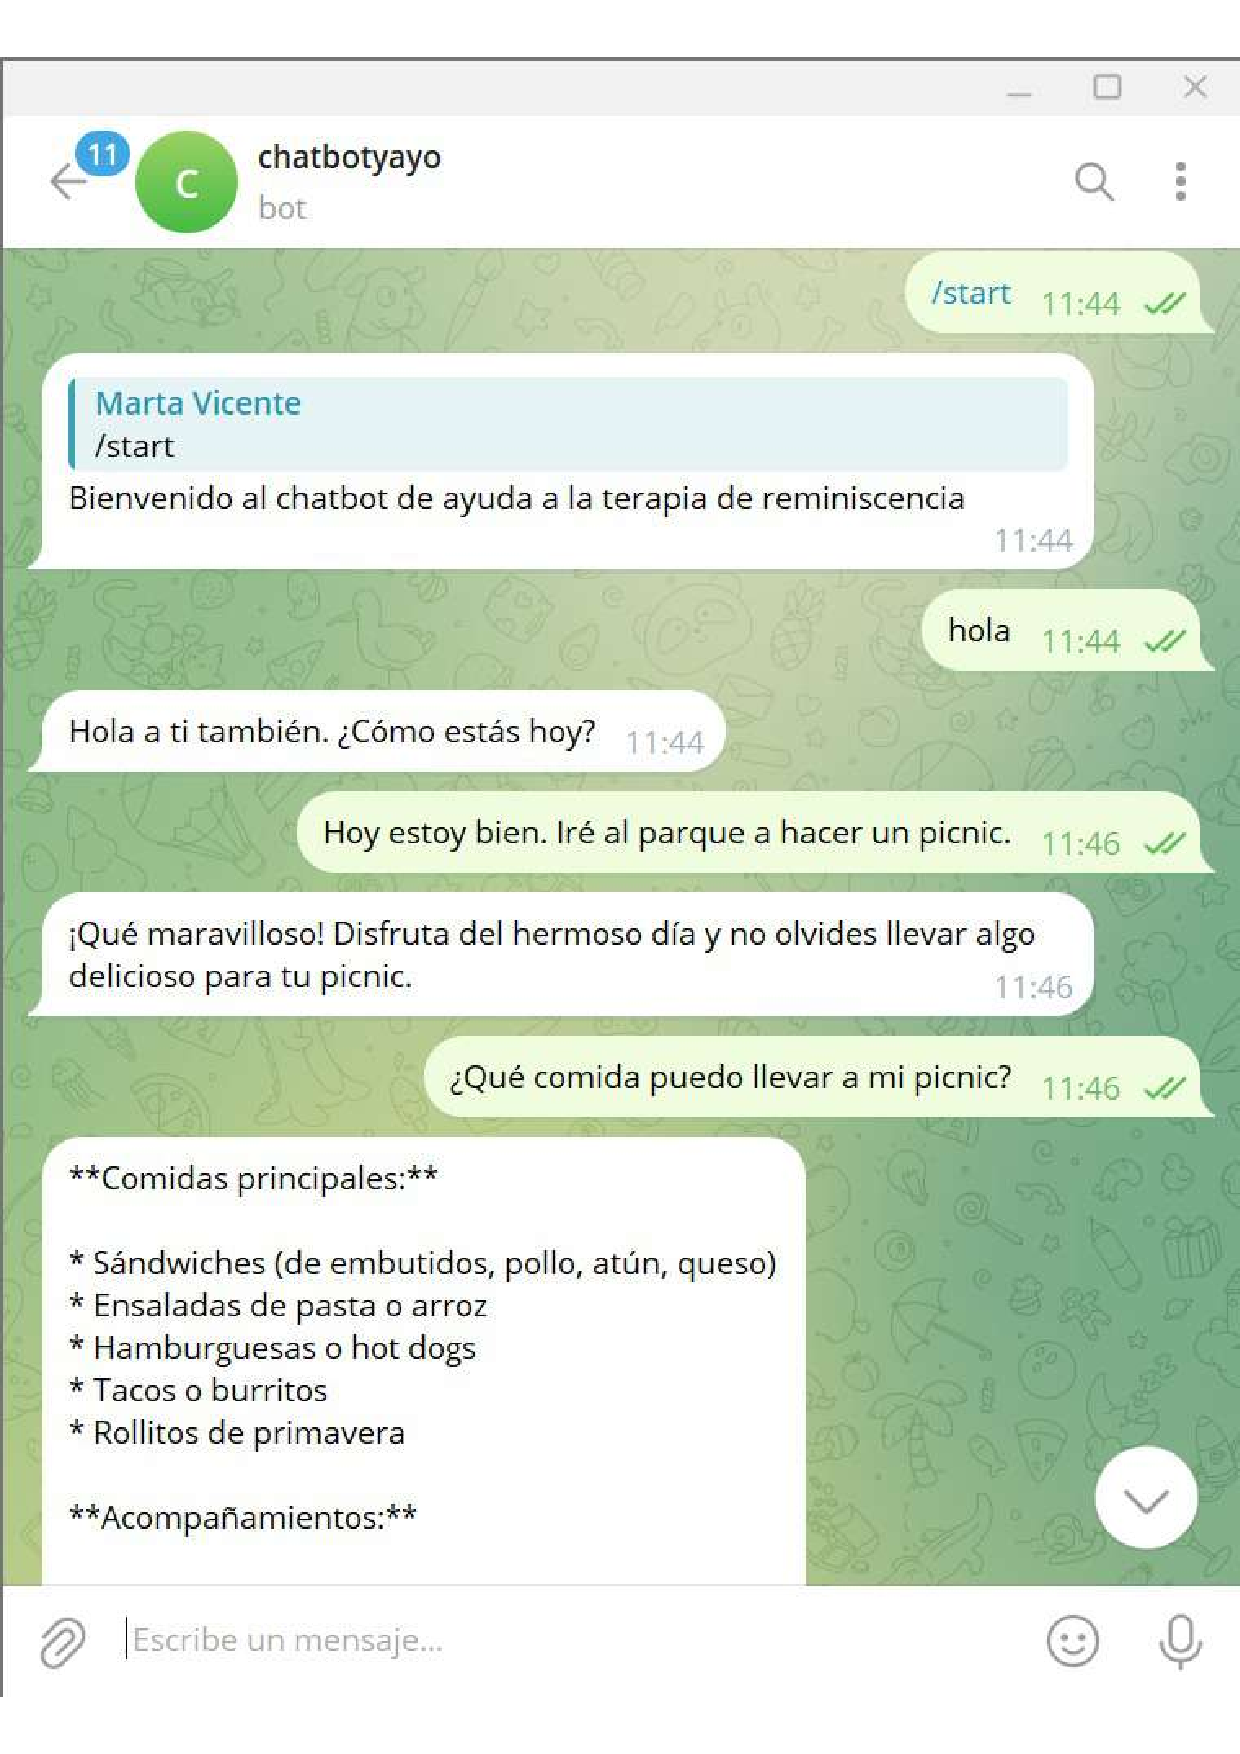
\includegraphics[width=0.5\textwidth]{Imagenes/telegram1}
